% !TeX program = lualatex
% !TeX encoding = UTF-8
% !TeX spellcheck = pt_BR
\documentclass[10pt, hyperref={pdfpagelabels=false}]{beamer}
\usepackage[utf8]{inputenc}
\usepackage[brazil]{babel}
\usepackage{lmodern}
\usepackage{url}
\usepackage{csquotes}

% Para fórmulas matemáticas
\usepackage{amsmath}
\usepackage{amssymb}
\usepackage{mathtools}

% Para setas usadas em fórmulas dos grafos
\usepackage{MnSymbol}

% Permite colocar figuras lado a lado ou
% fazer posicionamentos arbitrários
%\usepackage[lofdepth,lotdepth]{subfig}

% Para inserir gráficos e imagens
\usepackage{graphicx}
% Diretório padrão para figuras
\graphicspath{ {images/} }

% Para poder fazer texto cortado (strikethrough)
\usepackage[normalem]{ulem}

\usetheme[progressbar=frametitle]{metropolis}
\usepackage{appendixnumberbeamer}

\usepackage{booktabs}
\usepackage[scale=2]{ccicons}

\usepackage{pgfplots}
\usepgfplotslibrary{dateplot}

\usepackage{xspace}
\newcommand{\themename}{\textbf{\textsc{metropolis}}\xspace}

% Notações matemáticas usadas com frequência no texto.
% Isso possui três vantagens:
% 1 - Dá menos trabalho digitar as fórmulas
% 2 - Dá mais consistência à notação no trabalho
% 3 - Se mudar de ideia qto à notação, é só trocar aqui
%     e o trabalho todo fica certo.
% Notação matemática
\newcommand{\R}{\mathbb{R}} % Reais
\renewcommand\vec{\mathbf} % vetor como negrito
\newcommand{\avg}[1]{\left\langle #1 \right\rangle} % ... média
\newcommand{\defn}{\coloneqq} % Usamos "=", ":=" ou "\equiv?"
\newcommand{\noloop}[1]{#1^\nlcirclearrowleft} % ... sem loops
% Redes direcionadas
\newcommand{\linkin}[1]{#1^\leftarrow} % ... entrada
\newcommand{\linkout}[1]{#1^\rightarrow} % ... saída
\newcommand{\linkboth}[1]{#1^\leftrightarrow} % ... direcionada
% Redes ponderadas e direcionadas
\newcommand{\win}{w^\leftarrow} % peso e direção de entrada
\newcommand{\wout}{w^\rightarrow} % peso e direção de saída
\newcommand{\weighted}[1]{#1^w} % ... com pesos
\newcommand{\weighteddir}[1]{#1^{w\rightarrow}} % ... com peso e direção
% Reciprocidade
\newcommand{\recin}[1]{#1^\leftlsquigarrow} % ... entrada não-recíproca
\newcommand{\recout}[1]{#1^\leadsto} % ... saída não-recíproca
\newcommand{\recboth}[1]{#1^\leftrightsquigarrow} % ... recíproca
% Capacidades
\newcommand{\capac}{\textit{cap}}

\title{Qualificação}
\subtitle{Um Estudo do Mapa de Carreiras da Empresa Vagas.com Usando Ciência de Redes}
% \date{\today}
\date{}
\author{Aluno: Ronie Uliana \\ Orientador: Prof. Dr. Leandro Nunes de Castro}
\institute{Universidade Presbiteriana Mackenzie}
% \titlegraphic{\hfill\includegraphics[height=1.5cm]{logo.pdf}}

\begin{document}

\maketitle

\begin{frame}{Conteúdo}
  \setbeamertemplate{section in toc}[sections numbered]
  \tableofcontents[hideallsubsections]
\end{frame}

%===================
\section{Introdução}
%===================

\begin{frame}[fragile, label=pessoas]{Pesquisador e o Orientador}

  \begin{alertblock}{Ronie Uliana}
    Mestrando, Mackenzista, ex-UNAERP, ex-VAGAS.com, 99ner, Arquiteto de Software, \textit{Aluno}.
  \end{alertblock}
  
  \begin{alertblock}{Prof. Doutor Leandro de Castro}
    Doutor, Mackenzista, Pai, referência em Computação Natural, Empreendedor, \textit{Orientador}.
  \end{alertblock}
\end{frame}

\begin{frame}[fragile, label=pesquisa]{A Pesquisa}
  Uma \alert{análise de dados exploratória} sobre movimentação de profissionais entre ocupações utilizando técnicas de \alert{Ciência de Redes} sobre a base de currículos da empresa VAGAS.com.
\end{frame}

\begin{frame}[fragile, label=objetivo]{Objetivo}
  Encontrar e propor \alert{hipóteses} plausíveis para características de movimentação profissional usando as observações que divergem do acaso.
\end{frame}

\begin{frame}[fragile, label=dados]{Dados}
  Currículos anonimizados da empresas VAGAS.com (Fevereiro/2017).
  
  \begin{itemize}
    \item 10 milhões de currículos;\\
    \item 23 milhões de experiências profissionais;\\
    \item 8.348 ocupações distintas.
  \end{itemize}
\end{frame}

%=========================
\section{Ciência de Redes}
%=========================

{
\setbeamercolor{background canvas}{bg=white}
\begin{frame}[label=conceitos-basicos]{Conceitos de Redes}
  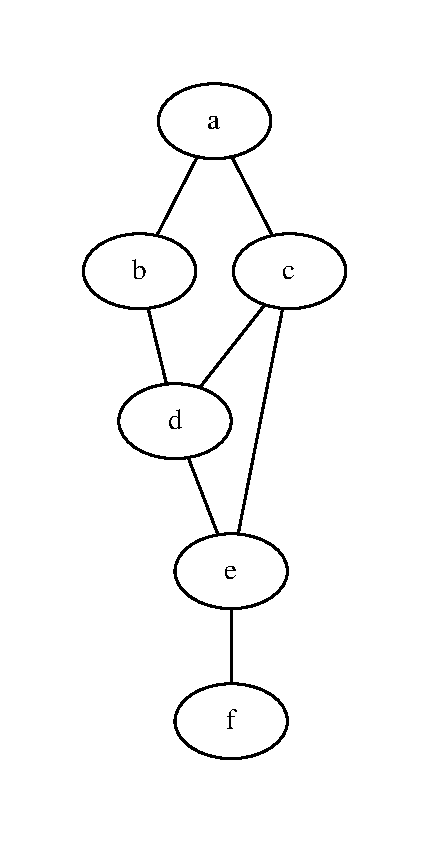
\includegraphics[width=0.2\textwidth]{simple.pdf}
  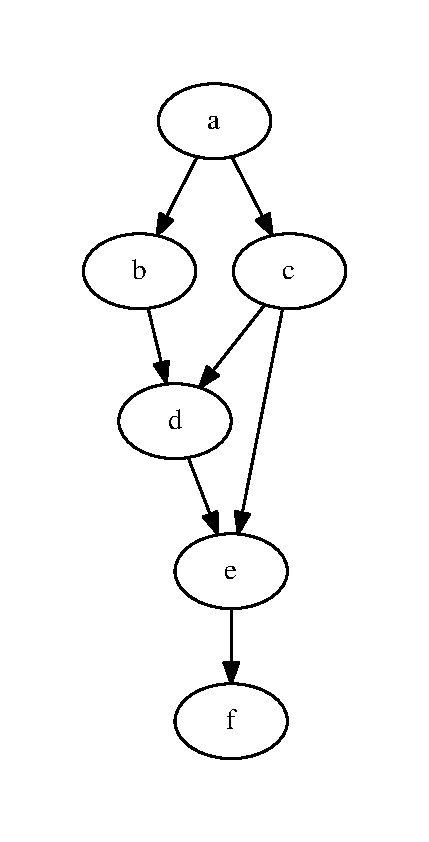
\includegraphics[width=0.2\textwidth]{directed.pdf}
  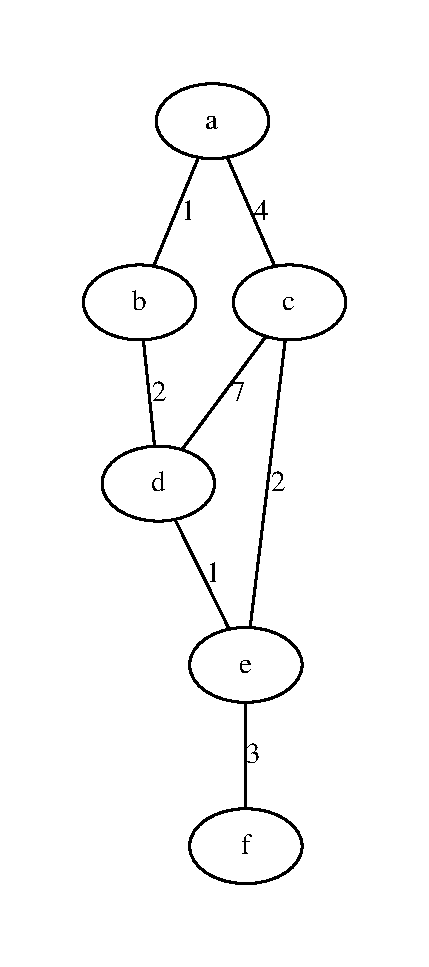
\includegraphics[width=0.2\textwidth]{weighted.pdf}
  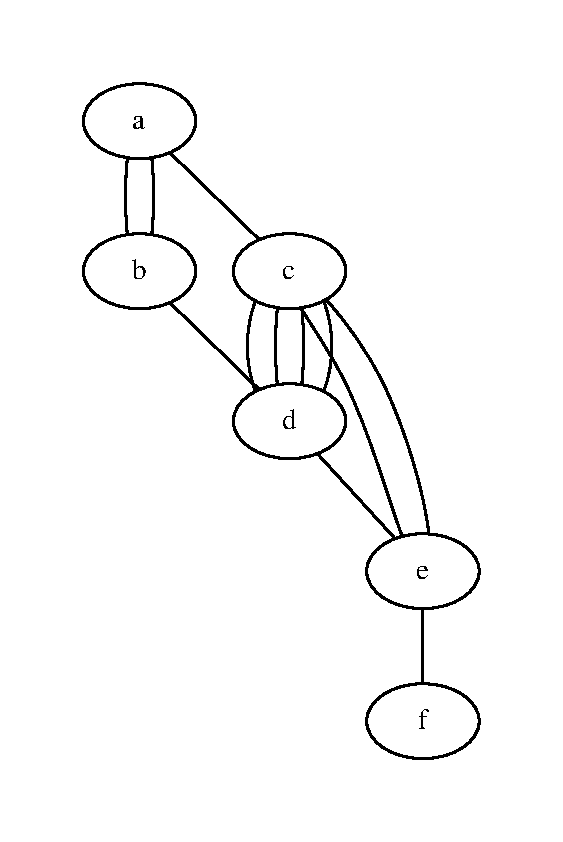
\includegraphics[width=0.2\textwidth]{multiple.pdf}
  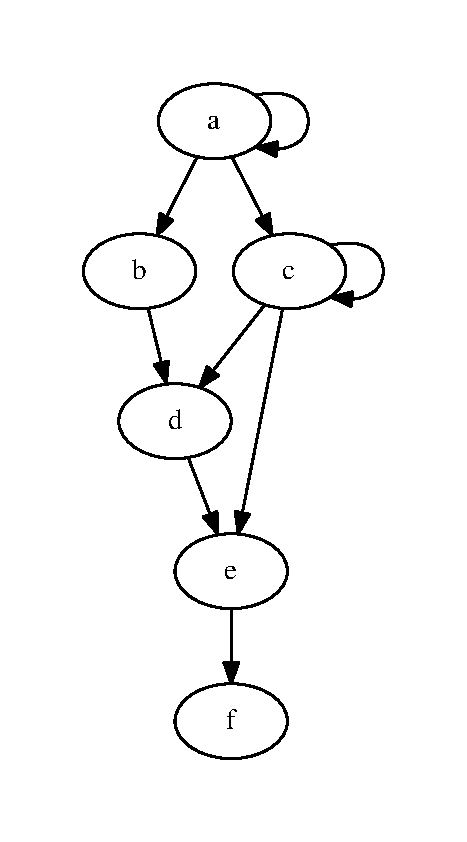
\includegraphics[width=0.2\textwidth]{loop.pdf}
\end{frame}
}

\begin{frame}[label=historia]{Breve História}
  \begin{itemize}
    \item Teoria de Grafos (Euler, século 18) - Matemática;
%    \item Redes Aleatórias (Erdős-Rényi/Gilbert, 1958) - Análise Combinatória e Estatística;
    \item Mundo Pequeno (Watts-Strogatz, 1998) - Popularização;
    \item Livre de Escala (Barabási-Albert, 1999) - Redes Complexas;
    \item Reconhecimento (USNRC, 2005) - \alert{Ciência de Redes}.
  \end{itemize}
\end{frame}

\begin{frame}[label=definicao]{Definição}
  National Research Council (2006)~\cite{National_Research_Council2006-lv}:
  \begin{quote}
    O estudo da representação em rede de fenômenos físicos, biológicos e sociais levando a modelos preditivos desses fenômenos.
  \end{quote}
  Barabási e Pósfai (2016)~\cite{Barabasi2016-rn}:
  \begin{itemize}
    \item Interdisciplinar;
    \item Empírica;
    \item Matemática e Quantitativa;
    \item Computacional;
  \end{itemize}
\end{frame}

\begin{frame}[label=redes]{Redes Aleatórias e Redes Reais}
Redes aleatórias são \alert{Modelos Nulos}, similares à hipótese nula em estatística.

Se uma característica observada em uma \alert{Rede Real} não aparece em uma \alert{Rede Aleatória} equivalente, deve existir um \alert{princípio organizacional} ausente no Modelo Nulo.
\end{frame}

\begin{frame}[label=medidas]{Medidas}
  O que caracteriza uma rede:
  \begin{itemize}
    \item Grau e Força;
    \item Distância Geodésica;
    \item Centralidade;
    \begin{itemize}
      \item Grau e Força;
      \item Intermediação;
    \end{itemize}
    \item Coeficiente de Agrupamento;
    \item Reciprocidade;
    \item Assortatividade, similaridade, modularidade.
  \end{itemize}
\end{frame}

\begin{frame}[label=propriedades]{Propriedades Topológicas}
  \begin{alertblock}{Mundo Pequeno}
    A distância geodésica esperada entre dois nós quaisquer é muito pequena.
  \end{alertblock}
  \begin{alertblock}{Livre de Escala}
    A rede possui poucos nós muito conectados (\textit{hubs}) e muitos nós pouco conectados.
  \end{alertblock}
\end{frame}

\begin{frame}[label=modelos-nulos]{Modelos Nulos}
  Algoritmos para geração de redes aleatórias com características específicas para serem \alert{Modelos Nulos}.
  \begin{description}
    \item[Erdős-Rényi/Gilbert] Base do modelo aleatório;
    \item[Preservação de Grau] Preserva o grau de cada nó;
    \item[Preservação de Força] Preserva a força de cada nó\footnote{Contribuição do autor};
    \item[Xulvi-Brunet e Sokolov] Assortatividade artificial.
    \item[Randomização de Força] Desassociação de força e grau\footnote{Contribuição do autor (em desenvolvimento)}.
  \end{description}
\end{frame}

\section{Mapa de Carreiras}

{
\setbeamercolor{background canvas}{bg=white}
\begin{frame}[label=mapa-visao-geral]{Visão Geral}
  \begin{center}
    Um grafo resumindo a trajetória profissional\\dos usuários do site VAGAS.com.br

    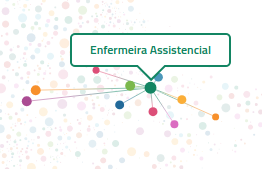
\includegraphics[width=0.4\textwidth]{mapa-enfermeira-assistencial}

  Cerca de \alert{10 milhões} de usuários\\resultando em \alert{8.348 ocupações} conectadas
  \end{center}
\end{frame}
}

\begin{frame}[label=mapa-construcao]{A Construção}
  \begin{center}
    Pipeline
    
    Processamento de texto
    
    Agrupamento de dados por ocupação
  \end{center}
\end{frame}

{
\setbeamercolor{background canvas}{bg=white}
\begin{frame}[label=mapa-dados]{Os Dados}
  Os dados disponíveis:

  \begin{columns}[T,onlytextwidth]
    \begin{column}{0.5\textwidth}
      \begin{itemize}
        \item Fluxo de profissionais
        \item Salários
        \item Tempo de Permanência
        \item Graduações
        \item Palavras-chave
      \end{itemize}
    \end{column}
    
    \begin{column}{0.5\textwidth}
      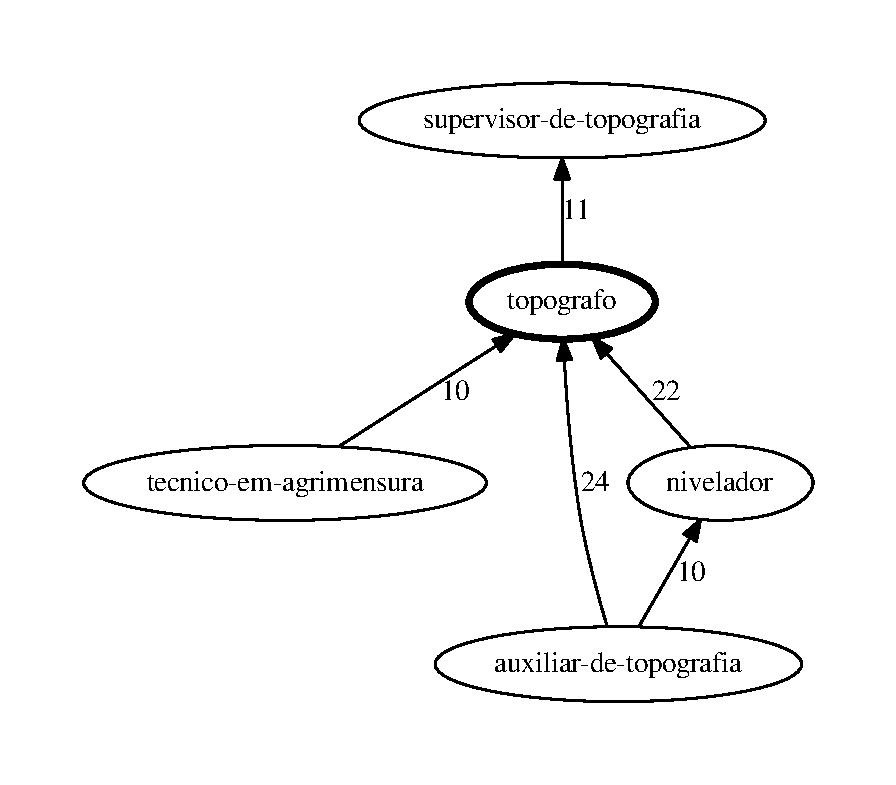
\includegraphics[width=\textwidth]{cluster_25}
    \end{column}
  \end{columns}
\end{frame}
}

\section{Resultados Parciais}

\begin{frame}[label=hipoteses]{As Hipóteses}
  \begin{enumerate}
    \item Atração Profissional
    \item \sout{Correlação Negativa entre Força de Entrada e a Mediana Salarial}
    \item Pontos de Saída do Mercado de Trabalho
    \item Pontos de Entrada do Mercado de Trabalho
    \item Trabalhos de Passagem 
    \item Equivalência Profissional 
    \item Detecção de Nomenclatura Equivalente 
    \item Capacitação Parcial
    \item Identificação de Carreiras
  \end{enumerate}
\end{frame}

\begin{frame}[label=hipotese-pontos-entrada-e-saida]{Pontos de Entrada e Saída}
  \begin{center}
    \begin{columns}[T,onlytextwidth]
      \begin{column}{0.5\textwidth}
        Variação da equação de reciprocidade:
        
        \begin{equation*}
          \recboth{s_i} \defn \frac{\linkin{s_i} - \linkout{s_i}}{s_i}
        \end{equation*}
        
        \begin{itemize}
          \item[] $s_i$ força do nó $i$
          \item[] $\linkin{s_i}$ força de entrada
          \item[] $\linkout{s_i}$ força de saída
        \end{itemize}
      \end{column}
    
      \begin{column}{0.5\textwidth}
        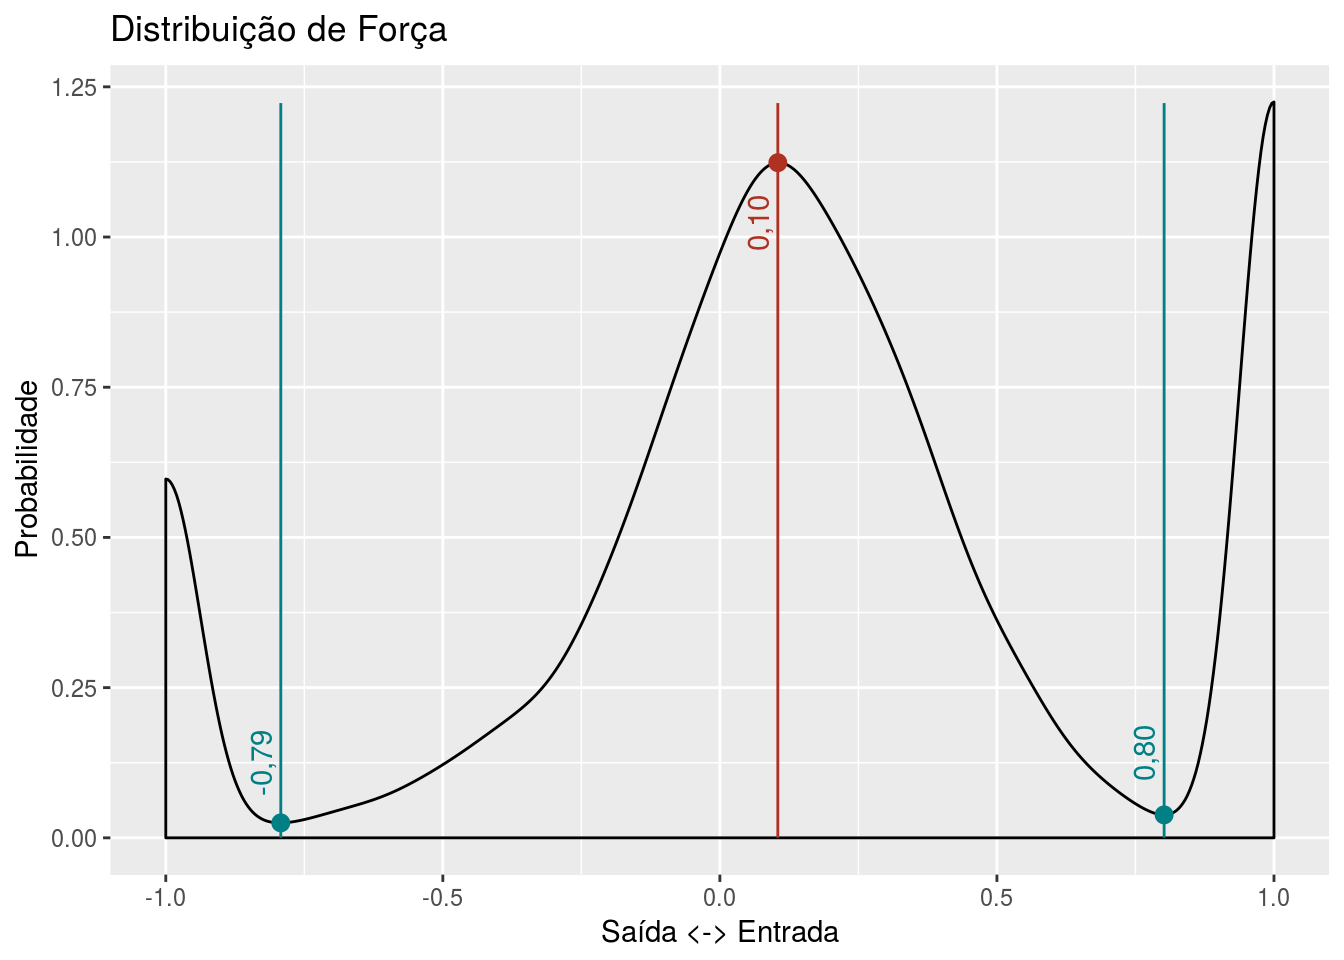
\includegraphics[width=\textwidth]{distribuicao-de-forca}
      \end{column}
    \end{columns}
  
    \vspace{\baselineskip}
  
    \textbf{-1} significa \enquote{somente saída} e \textbf{1} significa \enquote{somente entrada}
  \end{center}
\end{frame}

\begin{frame}[label=hipotese-ponto-de-saida-tabela]{Pontos de Saída}
  \begin{center}
    Ocupações com $\recboth{s_i}$ no \textit{limiar de saída}
    
    \vspace{\baselineskip}
    
    \begin{tabular}{l|c|c|c|c}
      \hline
      Ocupação & $s_i$ & $\linkin{s_i}$ & $\linkout{s_i}$ & $\recboth{s_i}$\\
      \hline
      analista desenvolvimento pesquisa & 111 & 101 & 10 & 0.82\\
      \hline
      analista gestao & 113 & 103 & 10 & 0.82\\
      \hline
      analista commerce & 126 & 115 & 11 & 0.83\\
      \hline
      coordenador unidade & 121 & 111 & 10 & 0.83\\
      \hline
      consultor investimento & 152 & 142 & 10 & 0.87\\
      \hline
      fonoaudiologo & 181 & 170 & 11 & 0.88\\
      \hline
    \end{tabular}
  \end{center}
\end{frame}


\begin{frame}[label=hipotese-ponto-de-entrada-tabela]{Pontos de Entrada}
  \begin{center}
    Ocupações com $\recboth{s_i}$ no \textit{limiar de entrada}
    
    \vspace{\baselineskip}
    
    \begin{tabular}{l|r|r|r|r}
      \hline
      Ocupação & $s_i$ & $\linkin{s_i}$ & $\linkout{s_i}$ & $\recboth{s_i}$\\
      \hline
      administrativo aprendiz jovem tecnico & 123 & 10 & 113 & -0.84\\
      \hline
      atendimento cliente profissional & 163 & 14 & 149 & -0.83\\
      \hline
      maquina moco & 138 & 12 & 126 & -0.83\\
      \hline
      embalador repositor & 143 & 13 & 130 & -0.82\\
      \hline
      equipe treinador & 185 & 17 & 168 & -0.82\\
      \hline
      aprendiz jovem mecanico & 135 & 13 & 122 & -0.81\\
      \hline
    \end{tabular}
  \end{center}
\end{frame}

\begin{frame}{Blocks}
  Three different block environments are pre-defined and may be styled with an
  optional background color.

  \begin{columns}[T,onlytextwidth]
    \column{0.5\textwidth}
      \begin{block}{Default}
        Block content.
      \end{block}

      \begin{alertblock}{Alert}
        Block content.
      \end{alertblock}

      \begin{exampleblock}{Example}
        Block content.
      \end{exampleblock}

    \column{0.5\textwidth}

      \metroset{block=fill}

      \begin{block}{Default}
        Block content.
      \end{block}

      \begin{alertblock}{Alert}
        Block content.
      \end{alertblock}

      \begin{exampleblock}{Example}
        Block content.
      \end{exampleblock}

  \end{columns}
\end{frame}


\begin{frame}{Line plots}
  \begin{figure}
    \begin{tikzpicture}
      \begin{axis}[
        mlineplot,
        width=0.9\textwidth,
        height=6cm,
      ]

        \addplot {sin(deg(x))};
        \addplot+[samples=100] {sin(deg(2*x))};

      \end{axis}
    \end{tikzpicture}
  \end{figure}
\end{frame}
\begin{frame}{Bar charts}
  \begin{figure}
    \begin{tikzpicture}
      \begin{axis}[
        mbarplot,
        xlabel={Foo},
        ylabel={Bar},
        width=0.9\textwidth,
        height=6cm,
      ]

      \addplot plot coordinates {(1, 20) (2, 25) (3, 22.4) (4, 12.4)};
      \addplot plot coordinates {(1, 18) (2, 24) (3, 23.5) (4, 13.2)};
      \addplot plot coordinates {(1, 10) (2, 19) (3, 25) (4, 15.2)};

      \legend{lorem, ipsum, dolor}

      \end{axis}
    \end{tikzpicture}
  \end{figure}
\end{frame}
\begin{frame}{Quotes}
  \begin{quote}
    Veni, Vidi, Vici
  \end{quote}
\end{frame}

{%
\setbeamertemplate{frame footer}{My custom footer}
\begin{frame}[fragile]{Frame footer}
    \themename defines a custom beamer template to add a text to the footer. It can be set via
    \begin{verbatim}\setbeamertemplate{frame footer}{My custom footer}\end{verbatim}
\end{frame}
}

\section{Conclusion}

\begin{frame}{Summary}

  Get the source of this theme and the demo presentation from

  \begin{center}\url{github.com/matze/mtheme}\end{center}

  The theme \emph{itself} is licensed under a
  \href{http://creativecommons.org/licenses/by-sa/4.0/}{Creative Commons
  Attribution-ShareAlike 4.0 International License}.

  \begin{center}\ccbysa\end{center}

\end{frame}

{\setbeamercolor{palette primary}{fg=black, bg=yellow}
\begin{frame}[standout]
  Questions?
\end{frame}
}

\appendix

\begin{frame}[fragile]{Backup slides}
  Sometimes, it is useful to add slides at the end of your presentation to
  refer to during audience questions.

  The best way to do this is to include the \verb|appendixnumberbeamer|
  package in your preamble and call \verb|\appendix| before your backup slides.

  \themename will automatically turn off slide numbering and progress bars for
  slides in the appendix.
\end{frame}

\begin{frame}[allowframebreaks]{References}

  \bibliography{main}
  \bibliographystyle{abbrv}

\end{frame}

\end{document}
